\section{Accuracy}
\label{sec:accuracy}

We test the models in \tablename{}~\ref{tab:models} on the test set, and get the accuracy from the Kaggle platform.
Results are listed in \figurename{}~\ref{fig:result-kaggle} and \figurename{}~\ref{fig:result-rrlda}.
The LDA model can achieve the best accuracy 94.47\%.
For reduced rank LDA, the test accuracy is much lower than the cross-validation accuracy.
This is because the test set samples are noised, and reduced rank LDA cannot tolerate noise.

\begin{figure}
    \centering
    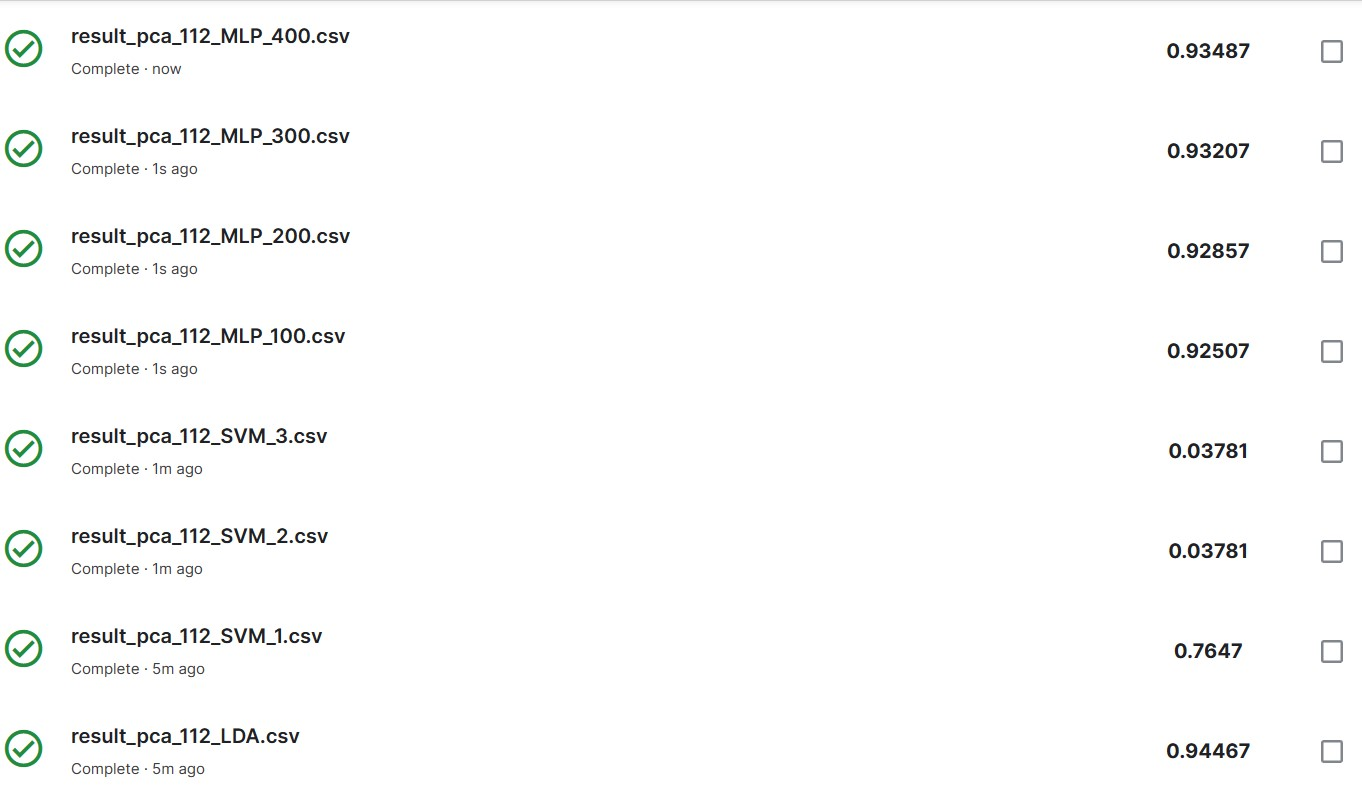
\includegraphics[width=\linewidth]{figures/kaggle.jpg}
    \caption{Accuracy result from Kaggle.}
    \label{fig:result-kaggle}
\end{figure}


\begin{figure}
    \centering
    
\includegraphics[width=\linewidth]{figures/rr-lda.jpg}
    \caption{Accuracy result of Reduced Rank LDA from Kaggle.}
    \label{fig:result-rrlda}
\end{figure}